% This is the Reed College LaTeX thesis template. Most of the work
% for the document class was done by Sam Noble (SN), as well as this
% template. Later comments etc. by Ben Salzberg (BTS). Additional
% restructuring and APA support by Jess Youngberg (JY).
% Your comments and suggestions are more than welcome; please email
% them to cus@reed.edu
%
% See http://web.reed.edu/cis/help/latex.html for help. There are a
% great bunch of help pages there, with notes on
% getting started, bibtex, etc. Go there and read it if you're not
% already familiar with LaTeX.
%
% Any line that starts with a percent symbol is a comment.
% They won't show up in the document, and are useful for notes
% to yourself and explaining commands.
% Commenting also removes a line from the document;
% very handy for troubleshooting problems. -BTS

% As far as I know, this follows the requirements laid out in
% the 2002-2003 Senior Handbook. Ask a librarian to check the
% document before binding. -SN

%%
%% Preamble
%%
% \documentclass{<something>} must begin each LaTeX document
\documentclass[12pt,twoside]{reedthesis}
% Packages are extensions to the basic LaTeX functions. Whatever you
% want to typeset, there is probably a package out there for it.
% Chemistry (chemtex), screenplays, you name it.
% Check out CTAN to see: http://www.ctan.org/
%%
\usepackage{graphicx,latexsym}
\usepackage{amsmath}
\usepackage{amssymb,amsthm}
\usepackage{longtable,booktabs,setspace}
\usepackage{chemarr} %% Useful for one reaction arrow, useless if you're not a chem major
\usepackage[hyphens]{url}
% Added by CII
\usepackage{hyperref}
\usepackage{lmodern}
\usepackage{float}
\floatplacement{figure}{H}
% End of CII addition
\usepackage{rotating}

% Next line commented out by CII
%%% \usepackage{natbib}
% Comment out the natbib line above and uncomment the following two lines to use the new
% biblatex-chicago style, for Chicago A. Also make some changes at the end where the
% bibliography is included.
%\usepackage{biblatex-chicago}
%\bibliography{thesis}


% Added by CII (Thanks, Hadley!)
% Use ref for internal links
\renewcommand{\hyperref}[2][???]{\autoref{#1}}
\def\chapterautorefname{Chapter}
\def\sectionautorefname{Section}
\def\subsectionautorefname{Subsection}
% End of CII addition

% Added by CII
\usepackage{caption}
\captionsetup{width=5in}
% End of CII addition

% \usepackage{times} % other fonts are available like times, bookman, charter, palatino


% To pass between YAML and LaTeX the dollar signs are added by CII
\title{Thesis}
\author{Emily Palmer}
% The month and year that you submit your FINAL draft TO THE LIBRARY (May or December)
\date{May 2018}
\division{Mathematics and Natural Sciences}
\advisor{Andrew Bray}
\institution{Reed College}
\degree{Bachelor of Arts}
%If you have two advisors for some reason, you can use the following
% Uncommented out by CII
% End of CII addition

%%% Remember to use the correct department!
\department{Mathematics}
% if you're writing a thesis in an interdisciplinary major,
% uncomment the line below and change the text as appropriate.
% check the Senior Handbook if unsure.
%\thedivisionof{The Established Interdisciplinary Committee for}
% if you want the approval page to say "Approved for the Committee",
% uncomment the next line
%\approvedforthe{Committee}

% Added by CII
%%% Copied from knitr
%% maxwidth is the original width if it's less than linewidth
%% otherwise use linewidth (to make sure the graphics do not exceed the margin)
\makeatletter
\def\maxwidth{ %
  \ifdim\Gin@nat@width>\linewidth
    \linewidth
  \else
    \Gin@nat@width
  \fi
}
\makeatother

\renewcommand{\contentsname}{Table of Contents}
% End of CII addition

\setlength{\parskip}{0pt}

% Added by CII

\providecommand{\tightlist}{%
  \setlength{\itemsep}{0pt}\setlength{\parskip}{0pt}}

\Acknowledgements{
I want to thank a few people.
}

\Dedication{
You can have a dedication here if you wish.
}

\Preface{

}

\Abstract{
The preface pretty much says it all. \par

Second paragraph of abstract starts here.
}

	\usepackage{tikz,amsmath}
% End of CII addition
%%
%% End Preamble
%%
%

\usepackage{amsthm}
\newtheorem{theorem}{Theorem}[chapter]
\newtheorem{lemma}{Lemma}[chapter]
\theoremstyle{definition}
\newtheorem{definition}{Definition}[chapter]
\newtheorem{corollary}{Corollary}[chapter]
\newtheorem{proposition}{Proposition}[chapter]
\theoremstyle{definition}
\newtheorem{example}{Example}[chapter]
\theoremstyle{definition}
\newtheorem{exercise}{Exercise}[chapter]
\theoremstyle{remark}
\newtheorem*{remark}{Remark}
\newtheorem*{solution}{Solution}
\begin{document}

% Everything below added by CII
  \maketitle

\frontmatter % this stuff will be roman-numbered
\pagestyle{empty} % this removes page numbers from the frontmatter
  \begin{acknowledgements}
    I want to thank a few people.
  \end{acknowledgements}

  \hypersetup{linkcolor=black}
  \setcounter{tocdepth}{2}
  \tableofcontents

  \listoftables

  \listoffigures
  \begin{abstract}
    The preface pretty much says it all. \par
    
    Second paragraph of abstract starts here.
  \end{abstract}
  \begin{dedication}
    You can have a dedication here if you wish.
  \end{dedication}
\mainmatter % here the regular arabic numbering starts
\pagestyle{fancyplain} % turns page numbering back on

\chapter{}\label{section}

\section{Introduction:}\label{introduction}

In the digital age data sets are everywhere. Billions of new data are
generated daily, in banking, social media, or in other scientific
studies. These data can be in numerous forms. With the availability of
the internet, text classification has become an interesting form of
data. While text classification problems are very frequent, similar
methods that instead classify music have not been explored as much.

Thinking of text or music as data has its own challenges. If we normally
think of data as something with lots of numbers in a spreadsheet, and
then running analysis on that spreadsheet. Analysis of text using
machine learning can find patterns, authors, or categories of text.
Similar methods can in fact be used to classify music.

The essential part of either text or music classification is feature
selection. Unlike in a data set of numerical or categorical values, text
and music must first go through a processing stage where hopefully
features of interest can be extracted before any models can be fit.

For music, th interest is in building a model that uses the extracted
features would be able to correctly classify a likely composer for that
piece of music. For musically trained humans, this might be an easy
task. Some are able to either by listening to a recording, or looking at
sheet music, automatically distinguish a piece composed by Bach or
Mozart. This becomes more difficult when composers are contemporaries.
Mozart and Saliery might be distinguishable to a scholar or music fan,
but it might be harder. Harder still is when a piece of music has a
disputed composer history. These examples exist throughout music
history, most notably in the Renaissance. Music classification has
attempted to assign composers to pieces to be disputed to be Josquin Des
Prez.

In both text and music classification, we must create features that can
be calculated that would give some signal to indicate some unconscious
tendendency of the composer that would make them distinguishable.

There have been numerous other interesting applications of machine
learning to music. Many studies have used neural nets etc trained on
composers music to have the computer create a similar composition.
\ldots{}.

\section{Brief history of text
classification}\label{brief-history-of-text-classification}

One of the earliest instances of text classification was on the
Federalist papers.(Mosteller \& Wallace, 1964). The famous Federalist
Papers were written under the pen name `Publius'. There are several
disputed papers attributed to James Madison or Alexander Hamilton. The
authors never admitted authorship, as some of the writings were
contradictory to their later political platforms. (Adair, 1944)
Historians have often examined the papers using styles of previously
known writings of Madison and Hamilton. Their analysis is often
partially based on the content of the letters, for example the existence
of citing English history is a trait more common to Hamilton. (Ford \&
Bourne, 1897)

In contrast, using the frequency of words such as and `by', `from', and
`upon', Mosteller and Wallace trained the writings on a set of known
writings by each author. These unconscious indicators were able to
differentiate between the two writers, and when a model was trained, the
model was able to identify the likely author of the disputed paper.

\section{Methods for classification.}\label{methods-for-classification.}

Initial approaches often use linear methods for classification. If we
are trying to predict the author,
\(y \in \{\text{Fanny},\text{Felix}\}\), or more generally,
\(y \in \{\text{list of composers}\}\), given features or predictors
\(\textbf{X} = \{X_{i \cdots X_p}\), we can divide the input space* into
a collection of regions labeled according to the classification.

We can create linear decision boundaries for \(K\) classes where the
fitted linear model for the \(k\)th indicator response is
\(\hat{f}_k(x) = \hat{\beta}_{k0} + \hat{\beta}_{k}^Tx.\) The decision
boundary between classes \(i\) and \(j\) is the set of points for which
\(\hat{f}_i(x) = \hat{f}_j(x)\), or in other words, the set
\(\{x : (\hat{\beta}_{i0} - \hat{\beta}_{j0}) + (\hat{\beta}_{i} - \hat{\beta}_j)^Tx = 0 \}\)
which defines a hyperplane.

Similarly quadratic decision boundaries can be used when we increase our
predictor space to include squares and higher polynomials of \(X\). We
then fit linear decision boundaries, which then map down to quadratic
functions in the original space.*.

Logistic regression is often used when the response is binary. It models
the probability that \(Y\) belongs to either category. We use the
logistic function
\(p(X) = \frac{e^{\beta_0 + \beta_1X}}{1 + e^{\beta_0 + \beta_1X}}\) To
calculate estimates of \(\hat{\beta_0},\hat{\beta_1}\), we use maximum
likelihood. To do this, we choose \(\hat{\beta_0},\hat{\beta_1}\) to
maximize the function \ldots{}

The Naive Bayes classifier is often used for musical classification as
it is good when the dimension \(p\) of the features space is large,
makeing density estimation unattractive*. It makes the (naive)
assumption that all the features are independent for a given class
\(i\). \[f_i(X) = \prod_{k = 1}^p f_{ik}(X_k)\]

The idea of separating Hyperplanes is essential to Support Vector
Machines (SVM)

Linear discriminant analysis: Using

GDA

\section{Feature selection}\label{feature-selection}

Text analysis, such as in the federalist papers, is read one word after
another. Information in piece of music, however, is read in a variety of
ways. It can be read left to right note by note, but it can also be read
vertically as the harmony, or the notes played together. Also in a piece
with several instruments, the above happens at the same time for each
instrument. There are also aspects that take place over large sections,
such as phrasing, or cadencial patterns. There are rules of counterpoint
that are followed throughout the entire piece. Thus we need to find
features that can be measured for each piece, or perhaps each measure or
instrument, that can describe a certain piece of music. Then we must
decide which features are those of rules and practices of classical
music, and where the creativeness and individuality of a composer
happens. As there are so many different aspects of a piece, the melodic
changes, harmonic ** etc, we can end up with very many (x) features to
describe one piece. As in this insteance when we only have
\textasciitilde{}150 total pieces, we have that \(p > n\). We thus need
to figure a clever way to decrease our predictor space. This can happen
in choosing what features we want to use to model, or using a dimension
reduction technique such as PCA.

Most of the musical stylometry papers have focused on composers in the
Renaissance, Baroque, and Classical eras. The Mendelssohns were
composing in the Romantic period. This choice might be because composers
in earlier eras followed rules of counterpoint more exactly, or perhaps
had less ``expressive'' allowances for their composing, thus making
features easier, although this is just speculation. There are also more
pieces with doubtful authorship in those eras. In addition Computer
Assisted Research in the Humanities (CCARH) has a large corpus of
encoded music from these times. * have a citation list of all the ones
that use these*

\section{A Very Short Introduction to Music
Theory}\label{a-very-short-introduction-to-music-theory}

Western sheet music is presented on a five line staff. The vertical
distance between notes (also known as an interval) depends on how many
half steps occur between two notes. There are 12 half steps in the
western scale. Melodic intervals are defined as the number of half steps
between two adjacent notes. Harmonic intervals are defined as the number
of half steps between notes played at the same time. Cadences are a type
of chord progresssion, usually occuring at the end of a phrase and
especially at the end of a piece. Musical notes are in the set
\(\text{note} \in \{A,B,C,D,E,F,G\}\) The value of a note can be changed
up or down a halfstep, by adding a sharp or flat. There are 12 unique
note value per octave. Intervals and chords can be either dissonant or
connsonant. Consonant intervals sound nice to our ears, whereas
dissonant intervals add a sense of tension or unease, which is used to
shape the feel of the music. In addition chords and intervals can be
minor or major. Minor intervals feel ``sad'', whereas major intervals
feel ``happy''.

\section{Musical features}\label{musical-features}

Features calculated from music often closely follow music theory. In
music, addition to deciding the features, there is also the decision of
the scope at where those features take place. They can be features for a
given instruemnt, the entire piece, or each measure. Also windowing
techniques can be used where a ``window'' is created over a given number
of bars or notes, and shifts accross the whole piece For each window, a
feature is recorded. These can be overlapping windows by creating an
``ofset'' of a number of beats or notes. This produces more data, as
instead of one feature for each piece, there is a feature for each
window.

Musical features are often thought about as either high level, or low
level. While the exact definition of each often varies, low level is
often understood to be features such as note frequency, etc. High level
features are more about a broader sense of the piece, including chord
progressions, etc. High level features are often what music experts use
in their analysis, whereas low-level features are more easily done with
computer analysis.

Especially in research regarding gene expression and text
categorization, data sets have enormous numbers of variables. We use
``feature'' and ``variable'' interchangably, with the exception when
features are created from variables, and the distinction will be made in
that case. (Guyon \& Elisseeff, 2003). There are several variable
selection algorithms that select the ``important'' variables. If we
included every variable that we extract from the piece, our model would
very likely be overfit.

The start of feature selection is domain knowledge. Thanks to John Cox
in the music department for suggesting a list of valuable features.
These will be described in Chapter 2.

\subsection{Background on Variable and Feature
Selection}\label{background-on-variable-and-feature-selection}

Often, especially in musical research, before analysis is done, numerous
features are extracted from the music without knowing a priori which
ones will be helpful in identifying a composers' style. Thus we have to
choose which features we want to use in our model. There are many ways
to do this. There are exissting variable selection algorithms that can
help with this process.

Several variable selection algorithms include variable ranking. Variable
ranking uses a score function to assign a score to each possible
variable. It is a computationally efficient method and is robust against
overfitting as it introduces bias but may result in less variance. It is
tempting to only include variables that have a high score. However, this
possibly leads to redundancy. In addition, variables that are not
important by themselves can have a significant performance improvement
when considered with other variables. Popular variable ranking methods
for classification are single variable classfiers and information
theoretic ranking criteria.

Single variable classifiers rank the variable according to thier
individual predictive power. The predictive power can be measured in
terms or error rate, or using the false positive or false negative rate
(fpr, fnr). This classifier cannot distinguish variables that perfectly
seperate the data.

The Information Theoretic Ranking Criteria is used in variable
selection. They often rely on estimates of the mutual information
between the predictor and response, as given by

\[ I(i) = \int_{x_i}\int_yp(x_i,y)\log\frac{p(x_i,y)}{p(x_i)p(y)}dxdy\]

where \(p(x_i)\) and \(p(y)\) are the probability densiites of \(x_i\)
the \(i^th\) predictor and \(y\) the response, and \(p(x_i,y)\) is the
joint density. \(I(i)\) is a measure of dependency between the density
of variable \(x_i\) and the density of the response \(y\) (reword)

After knowing the ranking of a variable we then select which variables
will be useful for our model. This is known as variable subset
selection. The three most common types of variable subset selection are
wrappers, filters, and embedded methods. Filters do not involve any
machine learning to create the criterian for varable subset selection.
Wrappers on the other hand use the ``performance of a learning machine
trained using a given feature subset.'' Embedded methods perform
variable selection in the process of training and are usually specific
to given learning machines

All possible subsets of variables is \(2^p-1\), which for large \(p\) is
often computationally impossible. Strategies like best-first, branch and
bound, simulated anealing, and genetic algorithms can help with the
computational difficulties.

Wrappers are often thought of as brute force methods. This can be good,
as it can reduce overfitting. Two types include forward selection and
backward elimination. These both give nested subsets of variables

Often there is a need for dimensionality reduction. Is there a way to
combine enough of the information given in the features in a smaller
dimensinoal space? This results in feature creationg; using the recorded
variables to create new features to fit the model on. These include
clustering, basic linear tranformations of the input variables, such as
PCa/SVd, and LDA. Also more sophistecated linear transformas like
Fourier and Hadamard. Two basic goals of these feature creations are
that we can achieve a good reconstruction of the data. The second is
that we can be most efficeint in making our predictors. The first is an
unsupervised problem. The second is supervised.

Clustering is in fact a type of feature construciton. The group of
clusterd points thereby becomes a feature. Examples of this include
K-means and hierarchical clustering.

\section{Previous research.}\label{previous-research.}

Research on musical stylometry focuses on two areas, data in the form of
audio, and data in the form of sheet music. Our analysis uses data in
the form of sheet music. To predict a composer, a training data set of
pieces of known composer is needed. Then that model can be fit to a
testing data set to predict composer. If that shows good predictions,
that model can be used on the pieces of unknown authorship.

Musical stylometry can be used disputed authorship, but also to detect
distinguishing musical styles of composer, even if there are no disputed
pieces. One such study did both. Backer et. al. first looked at
differences in style between J.S. Bach, Telemann, and Handel,Haydn and
Mozart. Next they looked at piece BWV 534 which is disputed to be
composed by either J.S. Bach, J.L. Krebs, or W.F. Bach (J.S. Bach's
son). (Backer \& Kranenburg, 2005)

\subsection{Previous choices of
features}\label{previous-choices-of-features}

Deciding on and extracting features of music is the first step to
analysis. Depending on the characteristics of the composer and time
period, different features would be useful. Often, features are
extracted en masse and then work is done later to determine which
features are important or useful in identifying style.

In addition to what kinds of features, in music there is also the
question of the scale at where those features take place. They can be
features for a given instruemnt, the entire piece, or each measure. Also
windowing techniques can be used where a ``window'' is created over a
given number of bars or notes, and moves thorugh the whole piece. For
each window, a feature is recorded. These can be overlapping windows by
creating an ``ofset'' of a number of beats or notes. This produces more
data, as instead of one feature for each piece, there is a feature for
each window, and there an be tens of windows in each piece.

Common types of features used before in music analysis are: Frequencies
or fractions of notes, chords, etc are a common low-level feature. These
include the fraction of the score that consisted of dissonant
sororities, as well as the fraction of bars that begin with a dissonant
sonority. Other features include the tipe of intervals or consonances
present in a piece: perfect consonance, imperfect consonances, and
dissonance. In polyphonic pieces, the four types of motion, (parallel,
similar, oblique, and contrary) can also be used as features.

Features measuring ``stability'' are also popular. Stability is computed
by dividing the standard deviation of the lengths of the fragment by the
mean length of the fragments. It is normalized in this way to be
comparable over differing time signatures. (Backer \& Kranenburg, 2005)

Markov transition matrices for the rhythms of the pieces, and Markov
transition matrices of the pitches in each piece

The above teqniques were used to analyze the music of Bach, Handel,
Telemann, Mozart and Haydn and compare J.S. Bach, W.F. Bach and J.L
Krebs in an attempt to classify BWV 534.(Backer \& Kranenburg, 2005)
They use overlapping windowing over each entire composition to produce
more data, and avoid issues of dimensionality. They chose a window of 30
bars to create a high enough number of fragments per piece and a low
enough variance of the feature values between fragments. They chose to
extract 20 features including features of freactions and measuring
stability, and entropy.

Aditionally, a number of previous papers have focused on Josquin des
Prez. This is likely due to the fact that there is a large training and
testing data set available in easily analyzable format provided by the
Josquin Research Project (citation). In addition there are a number of
pieces of disputed authorship that have been attributed to him. Work by
Brinkman et al. (Brinkman, Shanahan, \& Sapp, n.d.) use machine learning
approaches to evaluate attribution of compositions by des Prez. They
used both high level and low level features. The high level features
were 9-8 suspensions, oblique motion, contrary motion, similar motion
and parallel motion. The low level features were average melodic
entropy, normalized pairwise variability index (?), and note-to-note
transition probabilities.

Work by Speiser and Gupta (Speiser \& Gupta, n.d.) analyzed Josquin and
his contemporaries to attempt to classify unknown works. They extracted
four categories of features, frequencies of individual notes,
frequencies of pairwise interval combinations between each of the
voices, Markov transition matrices for the rhythms of the pieces, and
Markov transition matrices of the pitches in each piece. In total, this
lead to a total of 3000 features.

Other work looking at renessance and baroque composers looked
specifically at differences in counterpoint. Since most composers in
that era for the most part followed the rules of counterpoint, there is
a question of if there are distinguising differences. Using counterpoint
movement types, dissonance distributions, parallel intervals of each
kind, and vertical interval distributions, a classifier using a WEKA
algorithm, as well as Naive Bayes and a Decision Tree was created that
correctly predicted composer 2/3 of the time. (Mearns, Tidhar, \& Dixon,
2010)

\subsection{Previous applications}\label{previous-applications}

Most of the previous research has needed to do some kind of feature
selection. A lot of features are extracted as a priori we don't know
which features are distinguishing.

A modification of a forward selection (Floating Forward Selection(cite))
was used to extract features in order to identify distinguishing style
between Bach, Handel, Telemann, Mozart, and Haydn, and then subsequently
classify the authorship of BWV 535. (Backer \& Kranenburg, 2005) Each
composer was compared via creating comparisons of all possible class
arrangements, ie (Bach)(Handel), (Bach)(Handel,Teleman), etc. The
algorithm extracted features for each class arrangement that
distinguished the groups the best. A decision boundry was used for Bach
and not Bach, on the features Diss Part, Par thirds, and stab time
slice. A k-nearest neibors classifier was successful in comparing Bach
and others as well as each individual composer. Decision trees to
interpret the features used in decision making of the different class
arrangements. To determine authorship of BWV 535, they train a quadratic
Bayesian classifier to distinguish J.S. Bach, W.F. Bach and J.L Krebs.
They again compare every possible class arrangement as potential
composers.

PCA was used to analyze the music of Bach, Handel, Telemann, Mozart and
Haydn and compare J.S. Bach, W.F. Bach and J.L Krebs in an attempt to
classify BWV 534.(Backer \& Kranenburg, 2005) Although only two PC's
accounted for most of the variance, 5 PCs were used to account for more
variance. Binary comparisions were used to compare composers. This
resulted in a relatively clear separation between Bach and Josquin. For
Josquin and his contemporaries, the PC's do not do as well a job of
separation. The results of the principal component analysis run on all
the composers, were used to train a classifier on all the composers.
First a k-nearest neighbor classifier was used. To accound for most of
the variance, 27 PCs were used. Next they trained a support vector
machine classifier with a radial kernel. Finally they used a decision
tree to determine which features were important in discerning the
composers.

Speiser and Gupta (Speiser \& Gupta, n.d.) scored each feature by the
mutual information of each features. They then chose the top 50 features
and ran GDA. They then ran PCA to attempt to remove some of the
dependencies associated with musical features. They first fit a Naive
Bayes for classification, but it had a large training error as the
independence assumption does not work well with musical data. Next they
used support vector machines with a Gaussian kernel and GCA learning
algorithms.

** insert picture **

\section{Fanny and Felix Mendelssohn}\label{fanny-and-felix-mendelssohn}

Most musical stylometry analysis focuses on music of the Renaissance and
Baroque period, as there are more questions of authorship in that
period. As the Romantic period is much more modern in comparison, there
are many more surviving records of original manuscripts that include the
composer.

Felix Mendelssohn, often considered a prodigy akin to Mozart, was a
prolific composer. Before he was fourteen years old, he had already
written over 100 compositions.

His lesser known sister Fanny Hensel was also a composer of incredible
skill. The two were very close, for many years training and studying
together. In their early education living in Berlin, Felix and Fanny
received the same musical education, first piano lessons by Madam Bigot,
a famous pianist esteemed by Haydn and Beethoven. Beginning in 1818,
Carl Friedrich Zelter, a somewhat removed student of Bach and the most
influential Berlin musician of the time, began to teach them both
composition. In addition to music, the children were tutored by some of
the finest scholars in Berlin in subjects such as languages, history,
and drawing. Goethe himself claimed that Fanny was ``as gifted as
Felix''. (Tillard, 1996)

As Fanny grew up, her father started implying that she should focus her
energy on the domestic sphere of her life. While the fact that she never
became a world famous composer and performer is often attributed to the
gender politics of her time, it is also likely due to her high class.
(Reich, 1991) Especially considering the anti-semetic feelings of the
time, and since the family had recently converted from Judaism to
Christianity, the family did not want any other unusual characteristic
such as a professional female composer to set them further apart from
``polite'' society.

Most of Fanny's available work are Lieder, short pieces of voice
accompanied by piano. They were accepted at the time as the more
feminine, domestic compositions, acceptable for women to compose. Her
brother moved on to more elaborate compositions such as operas and
orchestral concertos. Her father pressured Fanny to remain composing
Lider. (Todd, 2003)
\begin{quote}
``Music will perhaps become his profession, while for you it can and
must only be an ornament, never the root of your being and doing. We may
therefore pardon him some ambition and desire to be acknowledged in a
pursuit which appears very important to him,\ldots{} while it does you
credit that you have always shown yourself good and sensible in these
matters; \ldots{} Remain true to these sentiments and to this line of
conduct; they are feminine, and only what is truly feminine is an
ornament to your sex.''
\end{quote}
Throughout their lives, Felix and Fanny maintained contact through
letters until Fanny's death in 1847 and Felix's death shortly
thereafter. These letters contain many instances of Felix asking for
advice on his compositions (include quote)

Unlike Felix who conducted and performed piano and organ in some of
Berlin's most esteemed concert halls, most of Fanny's performances were
private, only performed in small circles of her friends and family at
intimate parties. Similarly, although she was quite a prolific composer,
under recommendation of her father Abraham Mendelssohn, and to a lesser
extent Felix, Fanny did not publish her work until later in her life. In
1846 after her fathers death and though her brothers disapproval, she
published her first collection of Lieder. Many of Fanny's unpublished
notebooks are in private collections and are inaccessible

However, it is widely speculated (known?) that some of Fanny's work was
published under her brother's name, Especially three pieces each in his
Op 8 and 9 lieder. Famously, when Felix met the Queen of England, she
sang Felix's Lied ``Italien'', and Felix had to admit that in fact, it
was his sister that had written it. In a letter to Felix, Fanny admits:
\begin{quote}
``I have just recently received a letter from Vienna, which contained
basically nothing but the question of whether ``On Wings of Song'' was
by me, and that I should really send a list of things that are running
about in the world disguised, it seems that they aren't clever enough
themselves to separate the wheat from the chaff.'' (Mace, 2013)
\end{quote}
As she never made such a list, we are left to wonder if there are any
other pieces of hers that have been published under her brothers name
and reputation.

This project will use Lieder of Fanny and Felix Mendelssohn. Most of the
available work by Fanny are Lieder, of which Felix also composed a great
deal. We will see if there is a determinable difference in style of
these siblings who grew up very close and received mostly the same
musical education. We will then look at the (disputed?) Op 8 and 9.
Additionally, using Lieder that have been decidedly written by Felix, we
will see if any other of his earlier publications could have potentially
been written by Fanny.

\chapter{}\label{section-1}

\section{About the data and conversion
process}\label{about-the-data-and-conversion-process}

\section{Pieces used}\label{pieces-used}

The majority of the pieces used in this paper were Lieder of Felix
Mendelssohn and Fanny Hensel. While both composers composed different
types of music, the majority of available scores from Fanny Hensel were
Lieder. Felix Mendelssohn composed many different styles of music,
orchestral, piano, etc. Fanny Hensel in contrast has an available
existing corpus of mostly Lieder, although she did compose many works
for solo piano and orchestra. Of Felix's music, Lieder of Op 8 (12), op
9 (12), op 19(6), op 34 (6), op 47 (6), op 57 (6), op 71 (6), and 6
pieces of Lied without opus numbers, also 56 lied without a collection.
A total of 116 pieces.

Of Fanny's music, 23 lieder were used from her Lieder without Name
collection, 10 from her wo kommst du her collection, and 10 from, a
total of 43 pieces.

Data from JS Bach was also used. These data were available in Kern Score
format. from the Center for Computer Assisted Research in the
Humanities. (CCARH). The pieces used were the Well tempered clavier.
These were written as training pieces and each book contains 24 pieces
with one in every possible key. These were chosen as the data were more
easily accessible (no scanning was required), and they were a similar
format as the Mendelssohn songs, written as for solo piano(or
harpsichord).
\begin{Shaded}
\begin{Highlighting}[]
\NormalTok{knitr}\OperatorTok{::}\KeywordTok{include_graphics}\NormalTok{(}\StringTok{"images/scorephoto.JPG"}\NormalTok{)}
\end{Highlighting}
\end{Shaded}
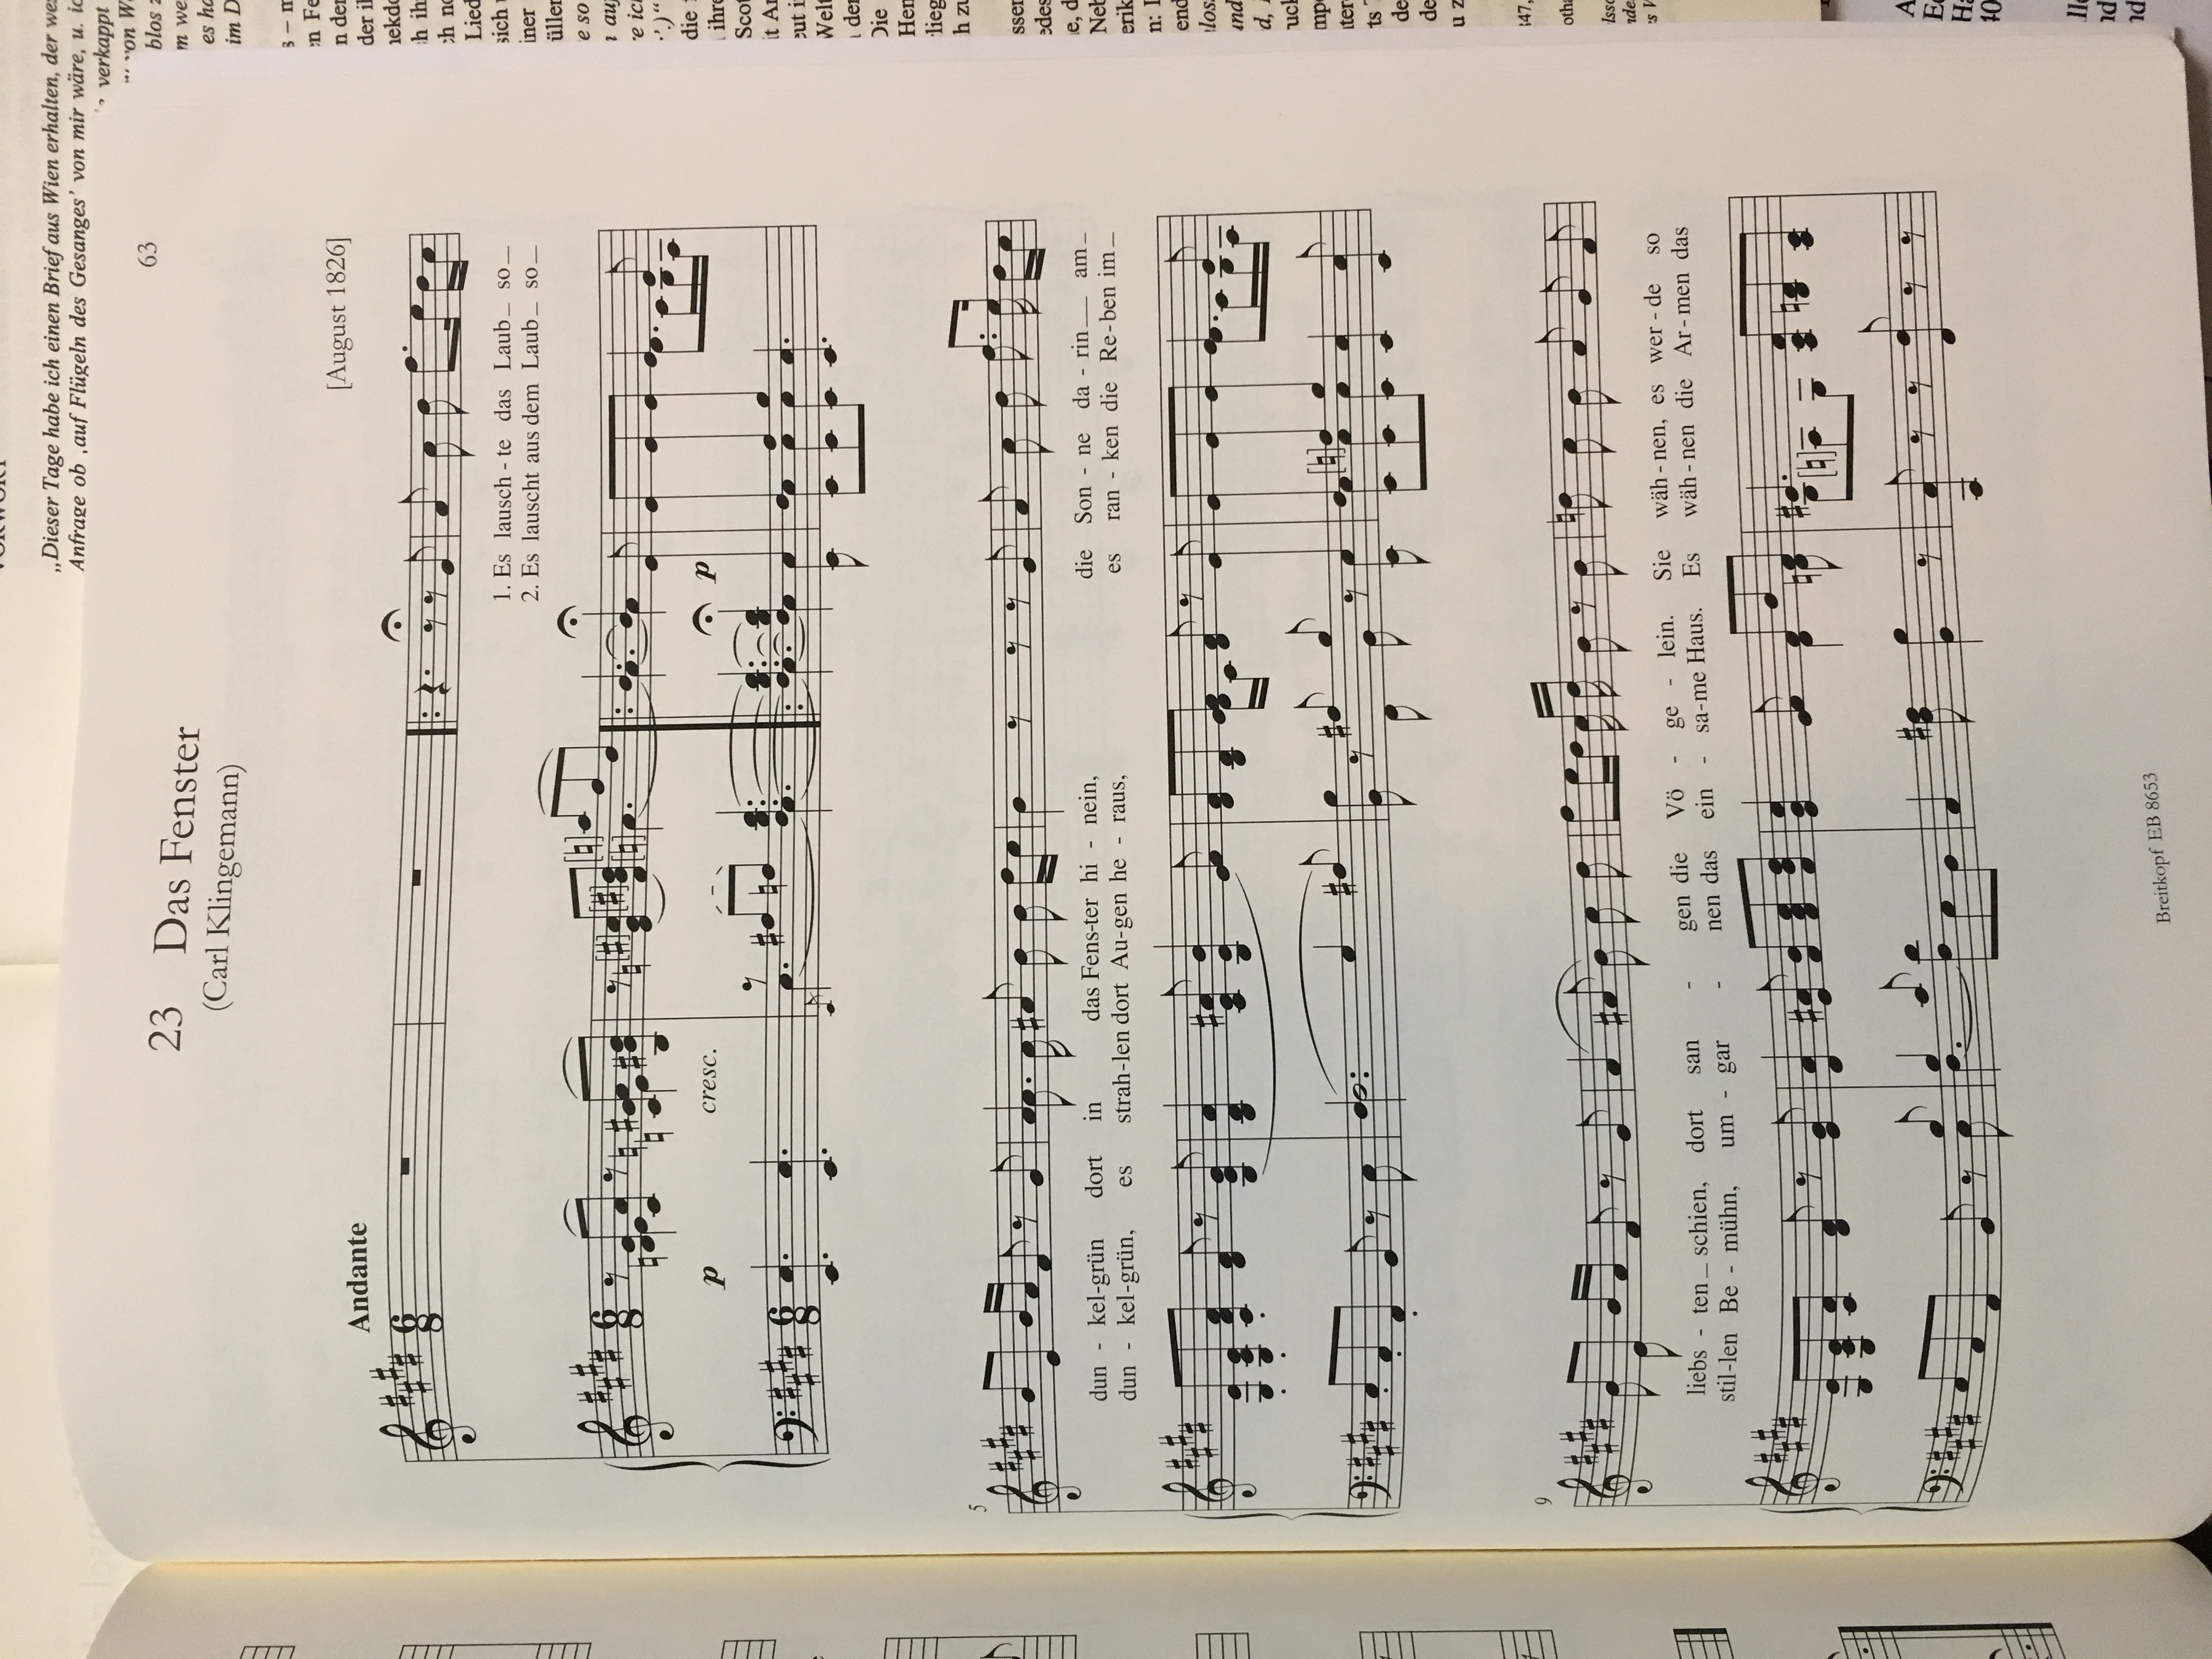
\includegraphics{images/scorephoto.JPG}

\section{Optical music recognition}\label{optical-music-recognition}

The vast majority of classical music is found solely in PDF or physical
copies. Sheet music as a form of data requires a lengthy process of
conversion before being able to be used in any analysis. Simply scanning
the scores into, say, a PDF, gives no musical semantics and can only be
viewed on screen or printed on paper. Thus, the two main steps in
reading in data from sheet music are: using optical music recognition
software to transform physical scores into digital formats, and to read
the digital format in to R where subsequent analysis can be done.

The scores used in this paper were obtained from physical copies
available in the Reed music library. These scores were then scanned
using software designed for optical music recognition (OMR).

Optical music recognition requires learning from graphical and textual
information. The main things the software must pick up are the locations
of bar lines, notes, rests, slurs, dynamic markings, tempo markings,
lyrics etc. Basic optical music recognition has been around since 1966.

Most commonly, the first step in optical music recognition is to remove
the staff lines. The staff lines are critical, as they define the basis
for the vertical definition distance of pitch, and the horizontal
distance definition of rhythm. The staff gives a normalization that is
helpful, essentially defining the size of what notes and rhythm look
like. Staff removal methods include projections, histograms, run
lengths, Candidates assemblage, contour tracking, and Graph path search.
(Doermann, Tombre, \& others, 2014)

The next step is music symbol extraction and classification. These
methods include template matching, where the object in question is
compared to existing known musical symbols, simple operators, such as
analysis of bounding boxes and projections, joining graphical
primitives, such as combining extracted objects such as notes, note
heads, and note beams to connect them in a musically correct way to form
chords etc. Other methods use statistical models for analyzing musical
primitives (the objects its trying to classify) such as Neural Networks,
Support Vector Machines, k-Nearest Neighbor, and Hidden Markov Models.

The next step OMR preforms is syntactical analysis and validation. This
step essentially uses defined grammars describing the organization of
music notation in terms of music symbols. This makes the classification
problem simpler, as there are existing rules and relationships between
musical symbols.
\begin{Shaded}
\begin{Highlighting}[]
\NormalTok{knitr}\OperatorTok{::}\KeywordTok{include_graphics}\NormalTok{(}\StringTok{"images/museScore.png"}\NormalTok{)}
\end{Highlighting}
\end{Shaded}
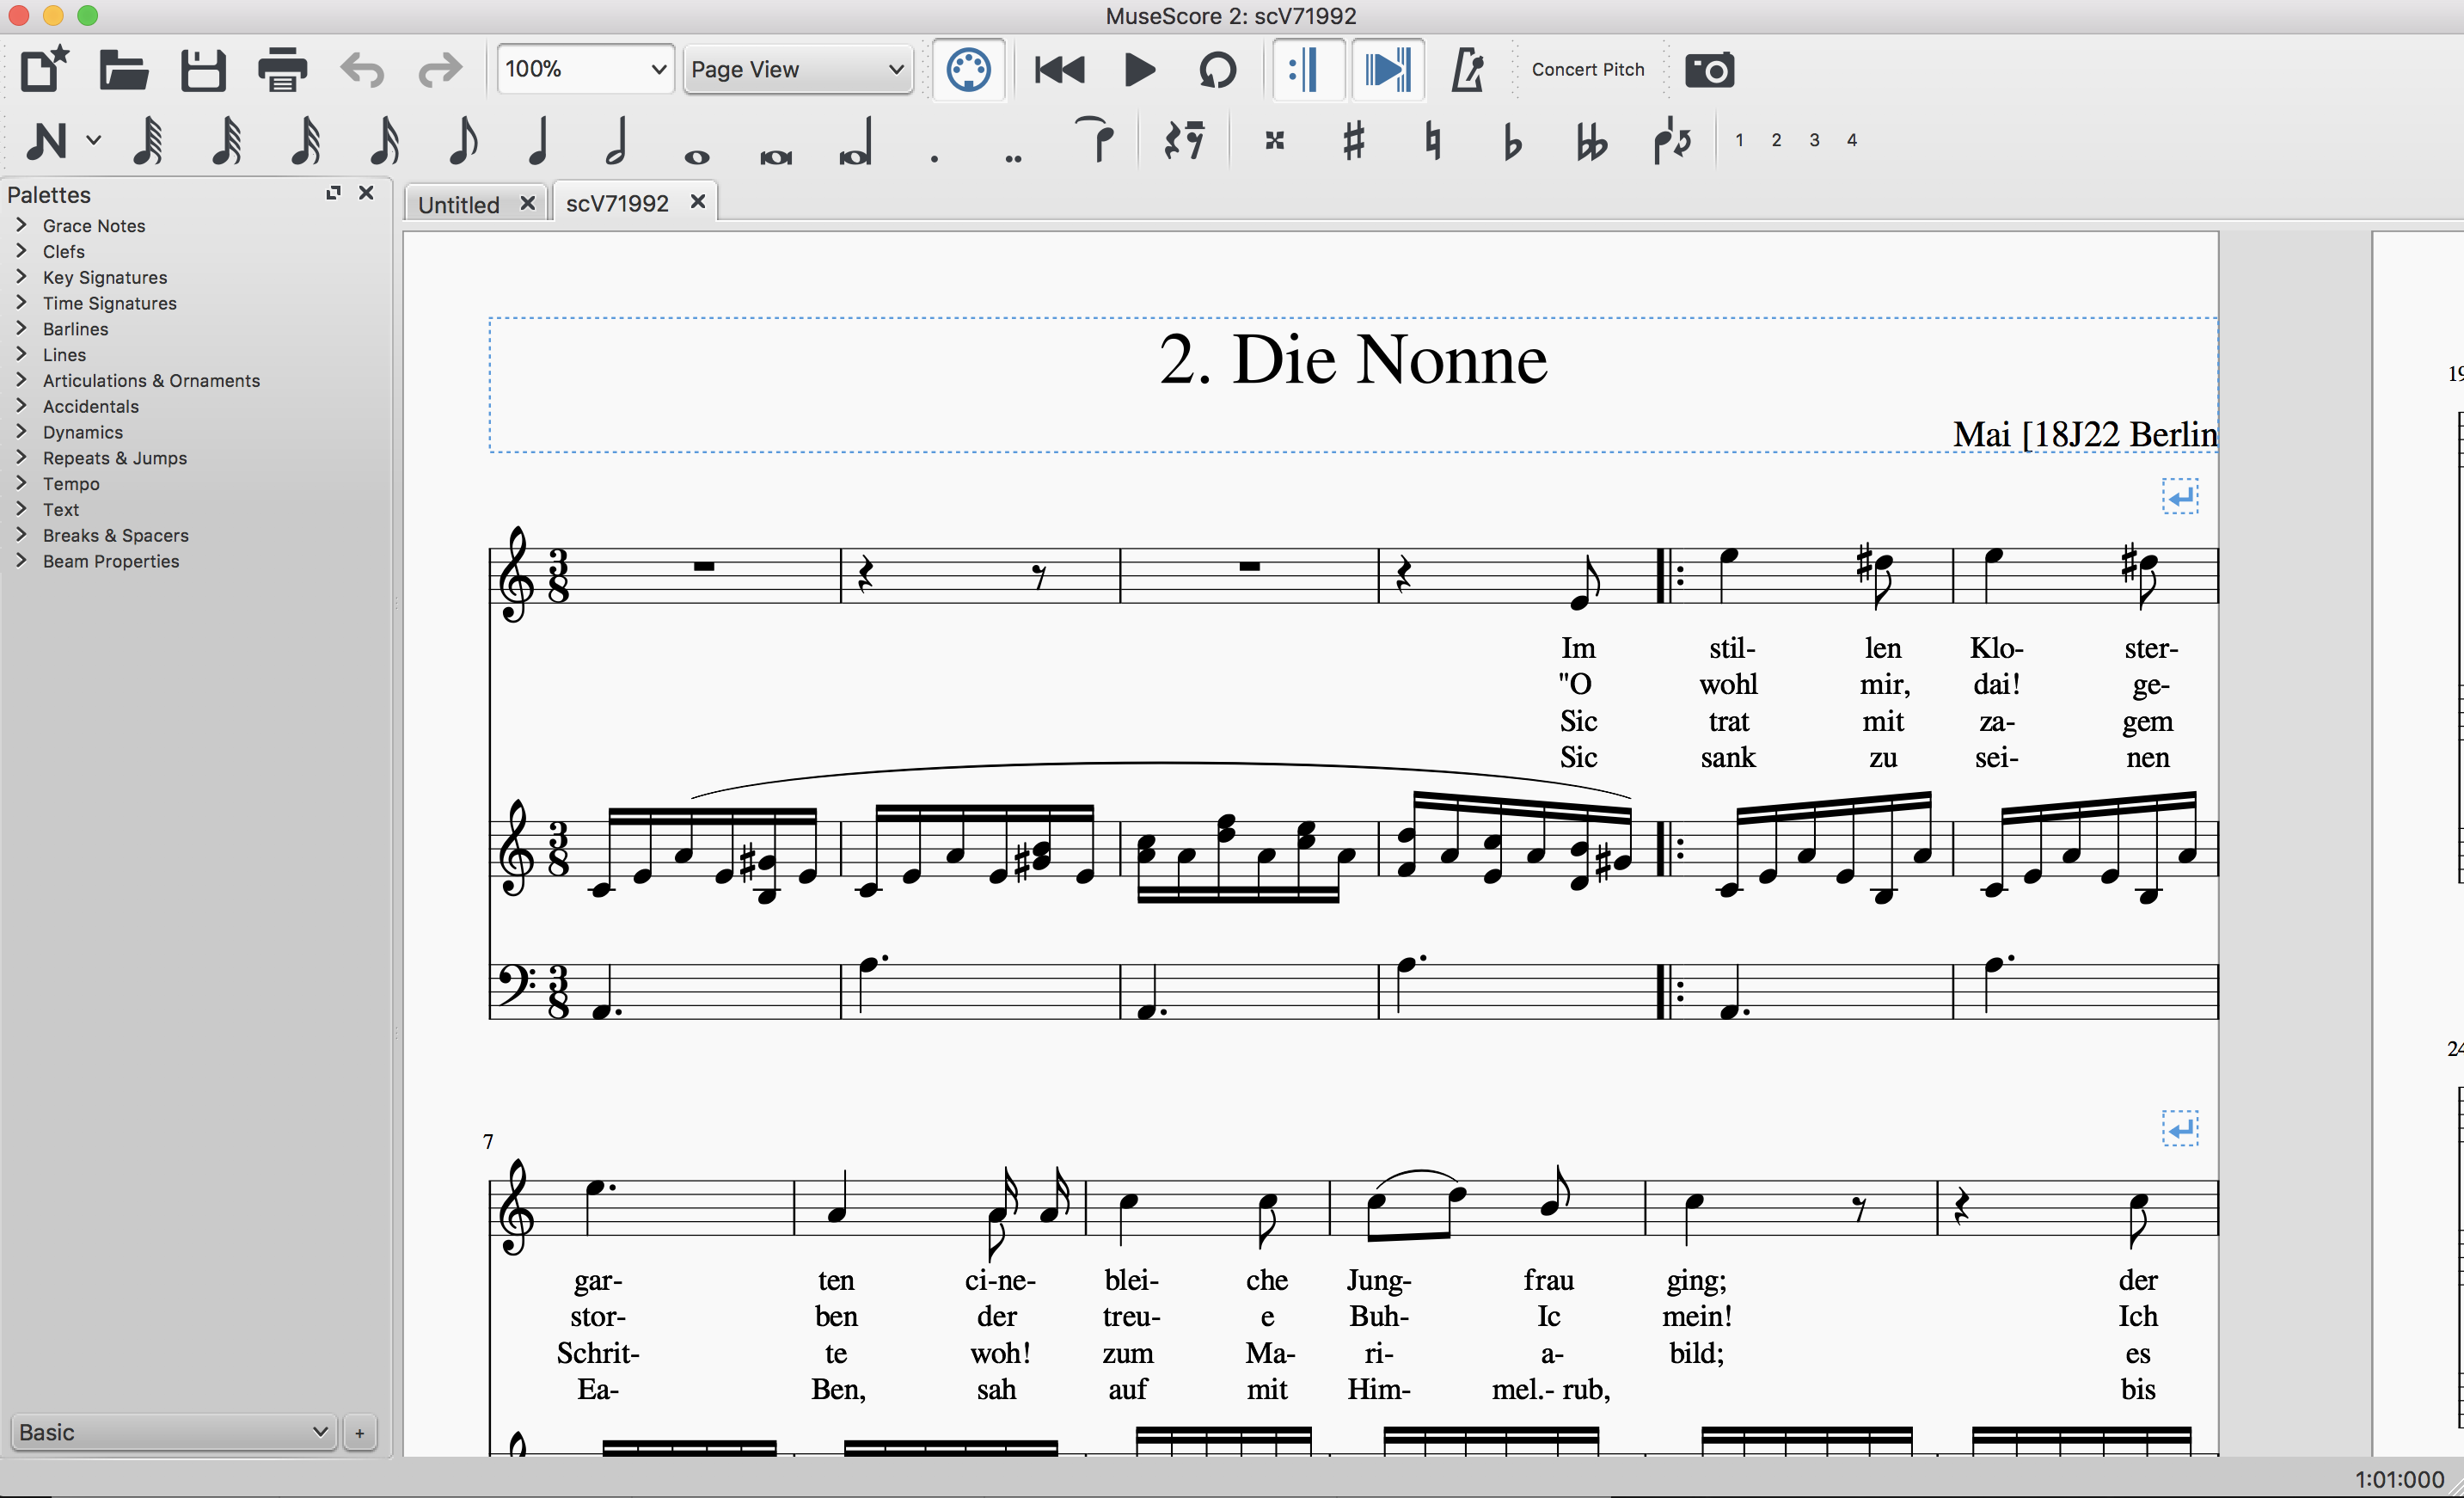
\includegraphics[width=400px]{images/museScore}

The OMR used in this paper was Photo Score. Photo Score works by
scanning the score on a flatbed scanner at a high resolution. It then
uses OMR techniques to output a musicXML file that can be read in by
most music composing software, such as Sibelius, Finale or Muse Score.
MusicXML is used commonly as a format for digital music, as it is
conducive to representing sheet music and music notation, and it can be
transferable to many different music software. Muse Score was chosen to
be the music software for viewing digital scores, as it is a free
software that can read MusicXML. After being read into Muse Score, each
piece was proof-read and corrected, as there were often errors in the
OMR, especially in recognizing triplets. Unfortunately, the scanning
process is very lengthy and time consuming, as the scanning often gives
a large number of mistakes. The score must be then scanned again. In
addition the proof-reading process is lengthy. We must check each note
and theme for errors against the original score, and change the
afflicted notes using Muse Score. The corrected score must then be
output as a musicXML file.

MusicXML on its own is not conducive to converting into a data frame as
representing the single half note middle C looks like this:
\begin{verbatim}
<?xml version="1.0" encoding="UTF-8" standalone="no"?>
<!DOCTYPE score-partwise PUBLIC
    "-//Recordare//DTD MusicXML 0.5 Partwise//EN"
    "http://www.musicxml.org/dtds/partwise.dtd">
<score-partwise>
  <part-list>
    <score-part id="P1">
      <part-name>Music</part-name>
    </score-part>
  </part-list>
  <part id="P1">
     <measure number="1">
      <attributes>
        <divisions>1</divisions>
        <key>
          <fifths>0</fifths>
        </key>
        <time>
          <beats>4</beats>
          <beat-type>4</beat-type>
        </time>
        <clef>
          <sign>G</sign>
          <line>2</line>
        </clef>
      </attributes>
      <note>
        <pitch>
          <step>C</step>
          <octave>4</octave>
        </pitch>
        <duration>4</duration>
        <type>whole</type>
      </note>
    </measure>
  </part>
</score-partwise> 
\end{verbatim}
We then need to convert into a format more easily readable into R. The
Kern Score music format is much more easily readable. The below picture
shows how a basic piece of music corresponds to a .krn file.
\begin{figure}
\centering
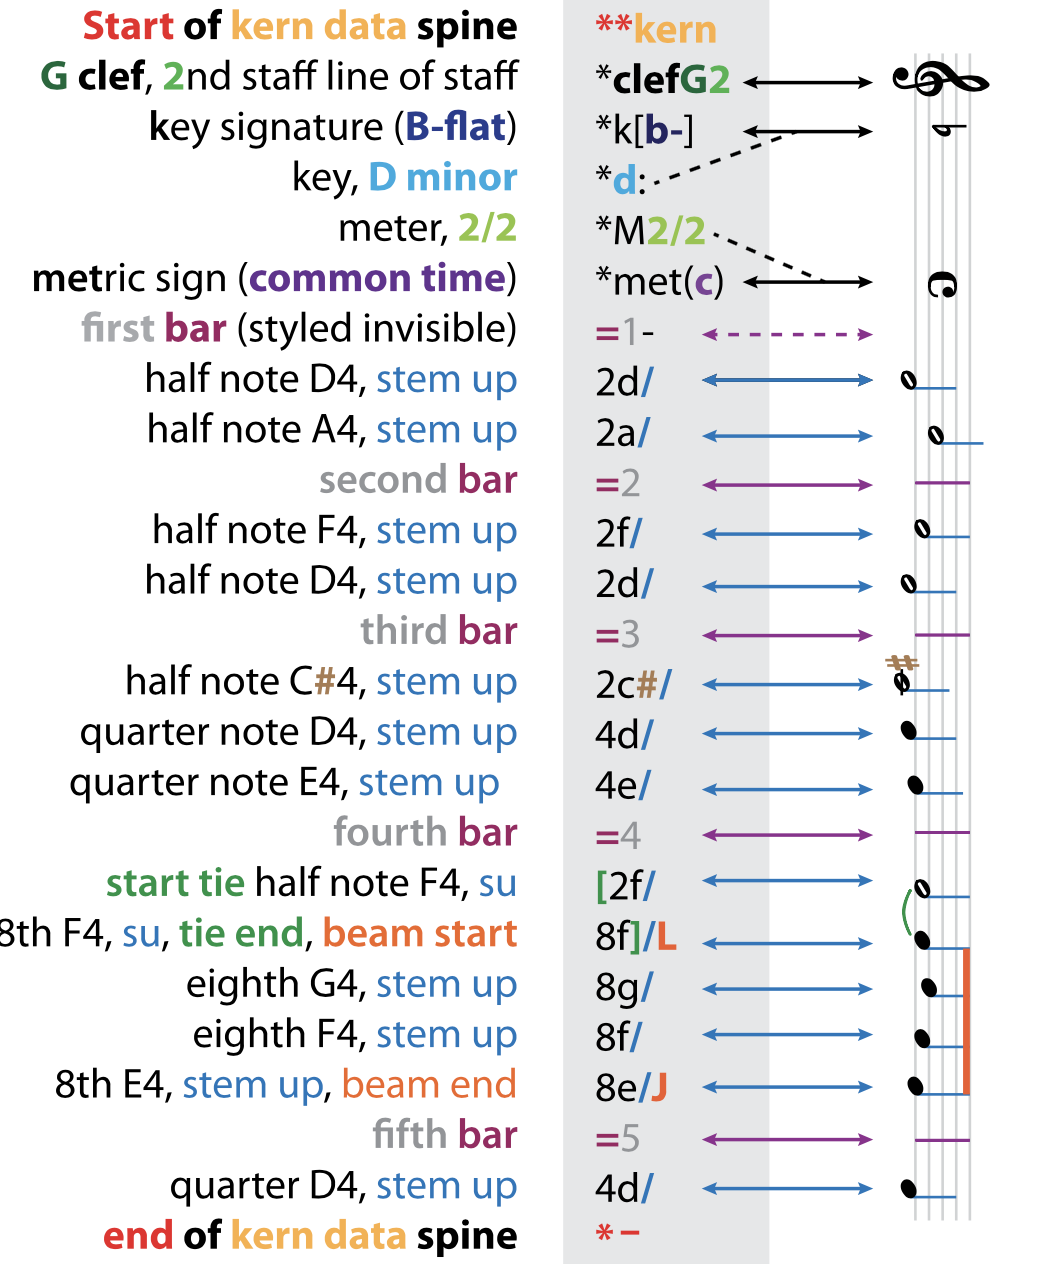
\includegraphics{images/krnmusic.png}
\caption{Shows how basic kern files correspond to sheet music}
\end{figure}
Each line of a krn file represents one value of a timebase. Kern files
are based on the smallest (shortest) rhythm value of a note found in a
piece. For example, if a piece was in 4/4 and there were sixteenth notes
present there would be 16*4 rows for each measure. The ``attack'' of
each note is the only note printed, the following time while the note is
held is represented with dots in the remaining rows until a new note is
sounded for that staff.

We do this by using Humdrum's function xml2hum that converts a musicXML
file into a .krn file. Humdrum is a computational music software. It is
a command line tool that has many functions for music analysis. The kern
file type can be read much more easily into R. Compared to above, the
code for a single middle c whole note would be :
\begin{verbatim}
**kern
*clefG2
*k[c]
*M4/4
=1-
1c/
\end{verbatim}
Each staff of a piece of music corresponds to one .krn spline. Each
spline is represented in a column. The lowest bass staff is the first
column and then progresses up to a soprano line.

The import\_xml\_files.sh file goes through the process of converting
scores from musicXML to .krn. The CCARH has a large data base mainly
baroque and Renaissance composers already in this format, which is where
the Bach data came from. The files that were scanned need to be
separated into having a separate file for each staff, which would mean a
seperate file for each instrument. In addition, since we are focused on
musical style, the text of the pieces are removed in this stage. In our
case for each piece there are always two or three files for each piece,
which are voice, piano right hand, and piano left hand. This is
necessary to avoid the bugs in xml2hum that have issues when staffs
don't necessarily match up as a result of the conversion process, most
often by rhythm.

\section{.krn to R}\label{krn-to-r}

Once we have .krn files to represent each piece we use regular
expressions to extract key information. For scanned music (Felix and
Fanny music), there are as many files are there are staffs, usually
three. MuseR's \texttt{krn2df()} and \texttt{piece\_df()} functions read
in .krn files and output a data frame in R for each piece. First the
data in .krn format are read in line by line using R's
\texttt{readLines()} function. This takes every line of the .krn file
and converts it into a vector. Each entry contains the rythem value and
note value. If there are multiple notes played at the same time, they
are all in one line. Then each entry is seperated out into the rythem
and note value for each note. Each line contains the following columns:
measure, rhythm value {[}4{]}, rhythm name {[}quarter note{]}, note
value {[}5{]}, note name (octave inclusive){[}cc{]}, note name (octave
exclusive){[} C sharp{]}. In addition, for the whole piece the key
signature and meter are recorded as columns.

A lot of data included in the .krn files are not necessary. For example,
we assume that whether or not a note has a step up or stem down offers
no help in classifying composer style, so this information is removed
when converting to an R data frame.

Inspired by the .krn file type, each row of the data frame contains one
time base value. For a given piece, the time base represents the
shortest note duration value. For example, if the shortest note a piece
contained was a sixteenth note, the time base would be 16. Each measure
then would contain 16 rows. This results in many rows of NA for certain
instruments, when a note is still being voiced, but it is not the
instance of the note being attacked.

\section{About the functions - MuseR}\label{about-the-functions---muser}

Once the scores are converted into R raw data, feature creation begins.
These features are mostly features suggested by John Cox.

To the best of my knowledge, there is currently no package of R that has
been built to analyze sheet music. There are existing packages (such as
tuneR) that examine audio formats of music. The intention of this thesis
was to create a package, museR, that takes sheet music in the proper
form (musicXML or .krn) and does all of the analysis using R.

\subsubsection{Melodic intervals}\label{melodic-intervals}

Melodic intervals, or the interval between two succesive notes, are
found using the \texttt{mel\_ints()} function. This first calculates the
top line of any instrument.

This outputs the proportion of each melodic interval happening over the
whole piece.

Similarly the \texttt{connsonance()} function outputs the proportion of
consonant (perfect, imperfect, dissonant) intervals over the whole piece
by calling \texttt{mel\_ints()}.

\subsubsection{Major\_minor}\label{major_minor}

For most musical analysis, the key of the piece is important in
determining chords, etc. The key is based on the key signature, which is
always given in a .krn file. Kern files from CCARH have the key of the
piece given, but

\subsubsection{Chords}\label{chords}

Suspended chords are currently not supported by MuseR. Chords that
begin, or are ``attacked'' at the same time count.

First, the key of the piece is found, as differnet chords depend on the
key. (really?)

Next, the times notes are played at the same time are extracted into a
list. Then the number of unique notes played at once is found. If there
are two notes played at once, \texttt{harm\_int()} calculates the
harmonic interval. This is done by calculating
\[note_1 - note_2 \mod(12)\] This gives the number of half steps between
each note. That number is then matched with the index of the interval.
Work is being done to have this include augmented and diminished
interval, but unfortunately that has not been completed at this time.

The possible triad chords are all defined by the intervals between each
note. For example, a Major triad is given by the base note, a major
third above the base, and a perfect fifth above the base. This
corresponds to 4 half steps then 4 half steps. Alternatively a minor
triad is given by the base, a minor third above, and a perfect fifth
aboe the base, which is 3 half steps, then 5 half steps.

A similar process is done for seventh chords.

\subsubsection{Resolutions}\label{resolutions}

\subsubsection{Density}\label{density}

\subsubsection{Par thirds, par fourths, par
sixths}\label{par-thirds-par-fourths-par-sixths}

\subsubsection{Prop scale degree}\label{prop-scale-degree}

\chapter{EDA}\label{eda}

\chapter{}\label{section-2}

\section{Feature Selection}\label{feature-selection-1}

Next they computed the entropy of the probability of occurrence of ways
of thinking about chords; chords are the same no matter what scale
degree they are on, and distinguishing chords differently. Next the
entropy was calculated given the probability of each pitch in the score.
Entropy was calculated by \(-\sum_{i = 1}^{N}p_i\log{p_i}\) where
\(p_i\) is the probability of occurrence, and \(N\) is the total
number.Next they the average number of active voices at one time. This
represents the voice density of the piece. Then for every interval, the
duration of that interval was divided by the total duration of all
intervals. Next the total duration of parallel thirds, fourths, and
sixths divided by the total duration of all intervals was measured.
Finally a measure of suspensions was found. (Backer)

\chapter{}\label{section-3}

\section{Model selection}\label{model-selection}

\chapter{}\label{section-4}

\section{Model Fit}\label{model-fit}

\chapter{}\label{section-5}

\section{Discussion}\label{discussion}

\chapter*{Conclusion}\label{conclusion}
\addcontentsline{toc}{chapter}{Conclusion}

If we don't want Conclusion to have a chapter number next to it, we can
add the \texttt{\{-\}} attribute.

\textbf{More info}

And here's some other random info: the first paragraph after a chapter
title or section head \emph{shouldn't be} indented, because indents are
to tell the reader that you're starting a new paragraph. Since that's
obvious after a chapter or section title, proper typesetting doesn't add
an indent there.

\appendix

\chapter{The First Appendix}\label{the-first-appendix}

This first appendix includes all of the R chunks of code that were
hidden throughout the document (using the \texttt{include\ =\ FALSE}
chunk tag) to help with readibility and/or setup.

\textbf{In the main Rmd file}
\begin{Shaded}
\begin{Highlighting}[]
\CommentTok{# This chunk ensures that the thesisdown package is}
\CommentTok{# installed and loaded. This thesisdown package includes}
\CommentTok{# the template files for the thesis.}
\ControlFlowTok{if}\NormalTok{(}\OperatorTok{!}\KeywordTok{require}\NormalTok{(devtools))}
  \KeywordTok{install.packages}\NormalTok{(}\StringTok{"devtools"}\NormalTok{, }\DataTypeTok{repos =} \StringTok{"http://cran.rstudio.com"}\NormalTok{)}
\ControlFlowTok{if}\NormalTok{(}\OperatorTok{!}\KeywordTok{require}\NormalTok{(thesisdown))}
\NormalTok{  devtools}\OperatorTok{::}\KeywordTok{install_github}\NormalTok{(}\StringTok{"ismayc/thesisdown"}\NormalTok{)}
\KeywordTok{library}\NormalTok{(thesisdown)}
\end{Highlighting}
\end{Shaded}
\textbf{In Chapter \ref{ref-labels}:}

\backmatter

\chapter*{References}\label{references}
\addcontentsline{toc}{chapter}{References}

\markboth{References}{References}

\noindent

\setlength{\parindent}{-0.20in} \setlength{\leftskip}{0.20in}
\setlength{\parskip}{8pt}

\hypertarget{refs}{}
\hypertarget{ref-adair1944}{}
Adair, D. (1944). The authorship of the disputed federalist papers.
\emph{The William and Mary Quarterly: A Magazine of Early American
History,} 98--122.

\hypertarget{ref-backer2005}{}
Backer, E., \& Kranenburg, P. van. (2005). On musical stylometry---a
pattern recognition approach. \emph{Pattern Recognition Letters},
\emph{26}(3), 299--309.

\hypertarget{ref-brinkman2016}{}
Brinkman, A., Shanahan, D., \& Sapp, C. (n.d.). Musical stylometry,
machine learning, and attribution studies: A semi-supervised approach to
the works of josquin.

\hypertarget{ref-OMR}{}
Doermann, D., Tombre, K., \& others. (2014). \emph{Handbook of document
image processing and recognition}. Springer.

\hypertarget{ref-authorshipfed}{}
Ford, P. L., \& Bourne, E. G. (1897). The authorship of the federalist.
\emph{The American Historical Review}, \emph{2}(4), 675--687. Retrieved
from \url{http://www.jstor.org/stable/1833983}

\hypertarget{ref-guyon2003}{}
Guyon, I., \& Elisseeff, A. (2003). An introduction to variable and
feature selection. \emph{Journal of Machine Learning Research},
\emph{3}(Mar), 1157--1182.

\hypertarget{ref-mace2013}{}
Mace, A. R. (2013). \emph{Fanny hensel, felix mendelssohn bartholdy, and
the formation of the`` mendelssohnian'' style} (PhD thesis).

\hypertarget{ref-mearns2010}{}
Mearns, L., Tidhar, D., \& Dixon, S. (2010). Characterisation of
composer style using high-level musical features. In \emph{Proceedings
of 3rd international workshop on machine learning and music} (pp.
37--40). ACM.

\hypertarget{ref-mosteller1964inference}{}
Mosteller, F., \& Wallace, D. (1964). \emph{Inference and disputed
authorship: The federalist}. Addison-Wesley.

\hypertarget{ref-reich1991}{}
Reich, N. B. (1991). The power of class: Fanny hensel. \emph{Mendelssohn
and His World}, 86--99.

\hypertarget{ref-CompStyleAttri}{}
Speiser, J., \& Gupta, V. (n.d.). Composer style attribution.
\emph{Project Report for CS}, \emph{229}.

\hypertarget{ref-tillard1996}{}
Tillard, F. (1996). \emph{Fanny mendelssohn}. Hal Leonard Corporation.

\hypertarget{ref-todd2003}{}
Todd, R. L. (2003). \emph{Mendelssohn: A life in music}. Oxford
University Press.


% Index?

\end{document}
